\section{Results and Discussion}
\label{sec:results_discussion}

This section discusses the main results obtained across the completed W3--W8 components. The project begins with model-based numerical validation and then moves toward empirical volatility analysis, calibration, volatility-surface interpretation, and volatility risk premium backtesting.

The results should be interpreted in stages. W3 and W4 validate the numerical pricing framework under controlled model parameters. W5 connects the framework to market data and realised variance. W6 evaluates whether a one-factor Heston model can jointly fit SPX and VIX-related instruments. W7 studies the structural difference between VIX and SPX volatility surfaces. W8 evaluates the practical behaviour of a volatility risk premium strategy across regimes.

\subsection{W3--W4 Numerical Validation}

The first numerical validation compares the Monte Carlo engine from W3 with the COS pricing engine from W4. Both methods price the same model-implied VIX call under the same Heston/CIR parameter set. The benchmark parameters are
\begin{equation}
v_0=0.04,\qquad
\kappa=2,\qquad
\theta=0.04,\qquad
\sigma_v=0.5,
\end{equation}
with option maturity
\begin{equation}
T=\frac{30}{365},
\end{equation}
risk-free rate
\begin{equation}
r=0.03,
\end{equation}
and VIX option strike
\begin{equation}
K=20.
\end{equation}

The Monte Carlo engine simulates Heston stock and variance paths, computes realised variance, validates the realised variance against the analytical variance swap strike, and prices the model-implied VIX call. The COS engine uses the characteristic function of terminal CIR variance and computes the same expected payoff through a Fourier-cosine expansion.

The comparison is summarised in Table~\ref{tab:cos_mc_comparison}.

\begin{table}[htbp]
\centering
\begin{tabular}{lcc}
\toprule
Quantity & Value & Interpretation \\
\midrule
COS price & 2.008969 & Characteristic-function-based estimate \\
Monte Carlo price & 1.984952 & Simulation-based estimate \\
Absolute difference & 0.024017 & Difference between pricing engines \\
Relative difference & 1.21\% & Difference relative to Monte Carlo price \\
\bottomrule
\end{tabular}
\caption{Comparison between COS and Monte Carlo prices for the model-implied VIX call.}
\label{tab:cos_mc_comparison}
\end{table}

The absolute difference is
\begin{equation}
\mathrm{AbsError}
=
|C_0^{COS}-C_0^{MC}|
=
0.024017,
\end{equation}
and the relative difference is approximately
\begin{equation}
\mathrm{RelError}
=
\frac{|C_0^{COS}-C_0^{MC}|}{C_0^{MC}}
\approx
1.21\%.
\end{equation}

This result supports the numerical consistency of the two independently implemented pricing engines. Exact equality is not expected because Monte Carlo contains sampling and time-discretisation error, while the COS method contains truncation, finite-series approximation, and payoff-integration error.

\subsection{W5 Market Data and Volatility Risk Premium Findings}

The W5 stage extends the project from synthetic model testing to market-data analysis. The data pipeline collects VIX index levels, SPX index data, VIX futures settlement data, and a risk-free rate proxy. From SPX returns, realised variance is computed, while implied variance is approximated from the VIX index.

The volatility risk premium is estimated as
\begin{equation}
VRP_t
=
\frac{1}{12}
\left(
\frac{VIX_t}{100}
\right)^2
-
RV_{t,t+1M}.
\end{equation}
A positive value indicates that implied variance exceeds subsequently realised variance.

The W5 results support several stylised facts. VIX rises sharply during stress episodes, realised variance increases after market shocks, and the volatility risk premium is generally positive during calm periods. However, crisis periods may compress or reverse the premium. This behaviour is consistent with the interpretation of volatility as an insurance-like asset class: investors pay for protection in normal periods, while volatility sellers are compensated for bearing crash risk.

The W5 analysis also identifies the 2020 COVID shock and the 2022 inflation shock as important stress periods. In such regimes, implied volatility rises sharply, realised variance catches up after market moves, and the relationship between VIX changes and SPX returns becomes strongly negative.

\subsection{W6 Calibration Trade-Off}

The W6 calibration results show that the one-factor Heston model faces a structural difficulty when fitting both SPX and VIX markets. The SPX-only calibration fits the SPX implied-volatility surface well, with an SPX IV RMSE of \(0.0159\), but produces a VIX futures RMSE of \(5.90\). In contrast, the VIX-only calibration improves the VIX futures RMSE to \(1.32\), but the SPX IV RMSE deteriorates to \(0.0711\).

The joint calibration with \(\alpha=0.50\) produces an SPX IV RMSE of \(0.0561\) and a VIX futures RMSE of \(1.33\). This solution is closer to the VIX-only calibration than to the SPX-only calibration, suggesting that the joint objective sacrifices SPX smile fit to preserve the VIX futures fit.

This trade-off is economically meaningful. The SPX volatility smile is strongly influenced by negative stock-variance correlation and volatility-of-volatility. The VIX futures curve is more sensitive to the variance level, long-run variance, and mean-reversion speed. A single variance factor cannot easily satisfy both requirements at once.

\subsection{W7 Volatility Surface Analysis}

The W7 component analyses the structural difference between VIX and SPX implied-volatility surfaces. VIX options are options written on the VIX index itself. Their implied volatility is often interpreted as volatility-of-volatility because it reflects market expectations about the magnitude of future VIX movements.

Under the CIR variance process, terminal variance \(v_T\) follows a scaled non-central chi-square distribution. Since this distribution is positive and right-skewed, the model-implied VIX inherits a right-skewed distribution. This provides a mathematical explanation for the positive skew observed in VIX option prices.

The W7 results show that VIX and SPX smiles have opposite skew directions. The VIX smile has positive skew, meaning that out-of-the-money VIX calls are relatively expensive. The SPX smile has negative skew, meaning that out-of-the-money SPX puts are relatively expensive. This contrast is summarised in Table~\ref{tab:w7_smile_comparison}.

\begin{table}[htbp]
\centering
\begin{tabular}{lll}
\toprule
Feature & VIX Options & SPX Options \\
\midrule
Skew direction & Positive/right skew & Negative/left skew \\
Expensive wing & OTM calls & OTM puts \\
Underlying tail & Fat right tail & Fat left tail \\
Main crisis exposure & Volatility spikes & Equity drawdowns \\
Model source & Non-central \(\chi^2\) variance distribution & Negative Heston correlation \(\rho\) \\
Investor behaviour & VIX calls as tail hedge & SPX puts as downside protection \\
\bottomrule
\end{tabular}
\caption{Structural comparison between VIX and SPX implied-volatility smiles.}
\label{tab:w7_smile_comparison}
\end{table}

The reported one-month VIX 25-delta risk reversal is approximately \(+11.49\) volatility points, while the corresponding SPX 25-delta risk reversal is approximately \(-9.55\) volatility points. The opposite signs confirm the different economic roles of the two option markets. VIX calls insure against volatility spikes, while SPX puts insure against market declines.

This result also connects W7 to the earlier Heston model discussion. Negative stock-variance correlation explains the SPX downside skew, while the positive and right-skewed distribution of terminal variance explains the VIX upside skew.

\subsection{W8 Volatility Risk Premium Backtest}

The W8 component evaluates the practical behaviour of a volatility risk premium strategy. The generated outputs include backtest plots, daily and monthly P\&L summaries, regime-level metrics, beta decomposition, and risk dashboards.

Figure~\ref{fig:w8_backtest} shows the cumulative behaviour of the W8 volatility risk premium backtest.

\begin{figure}[htbp]
    \centering
    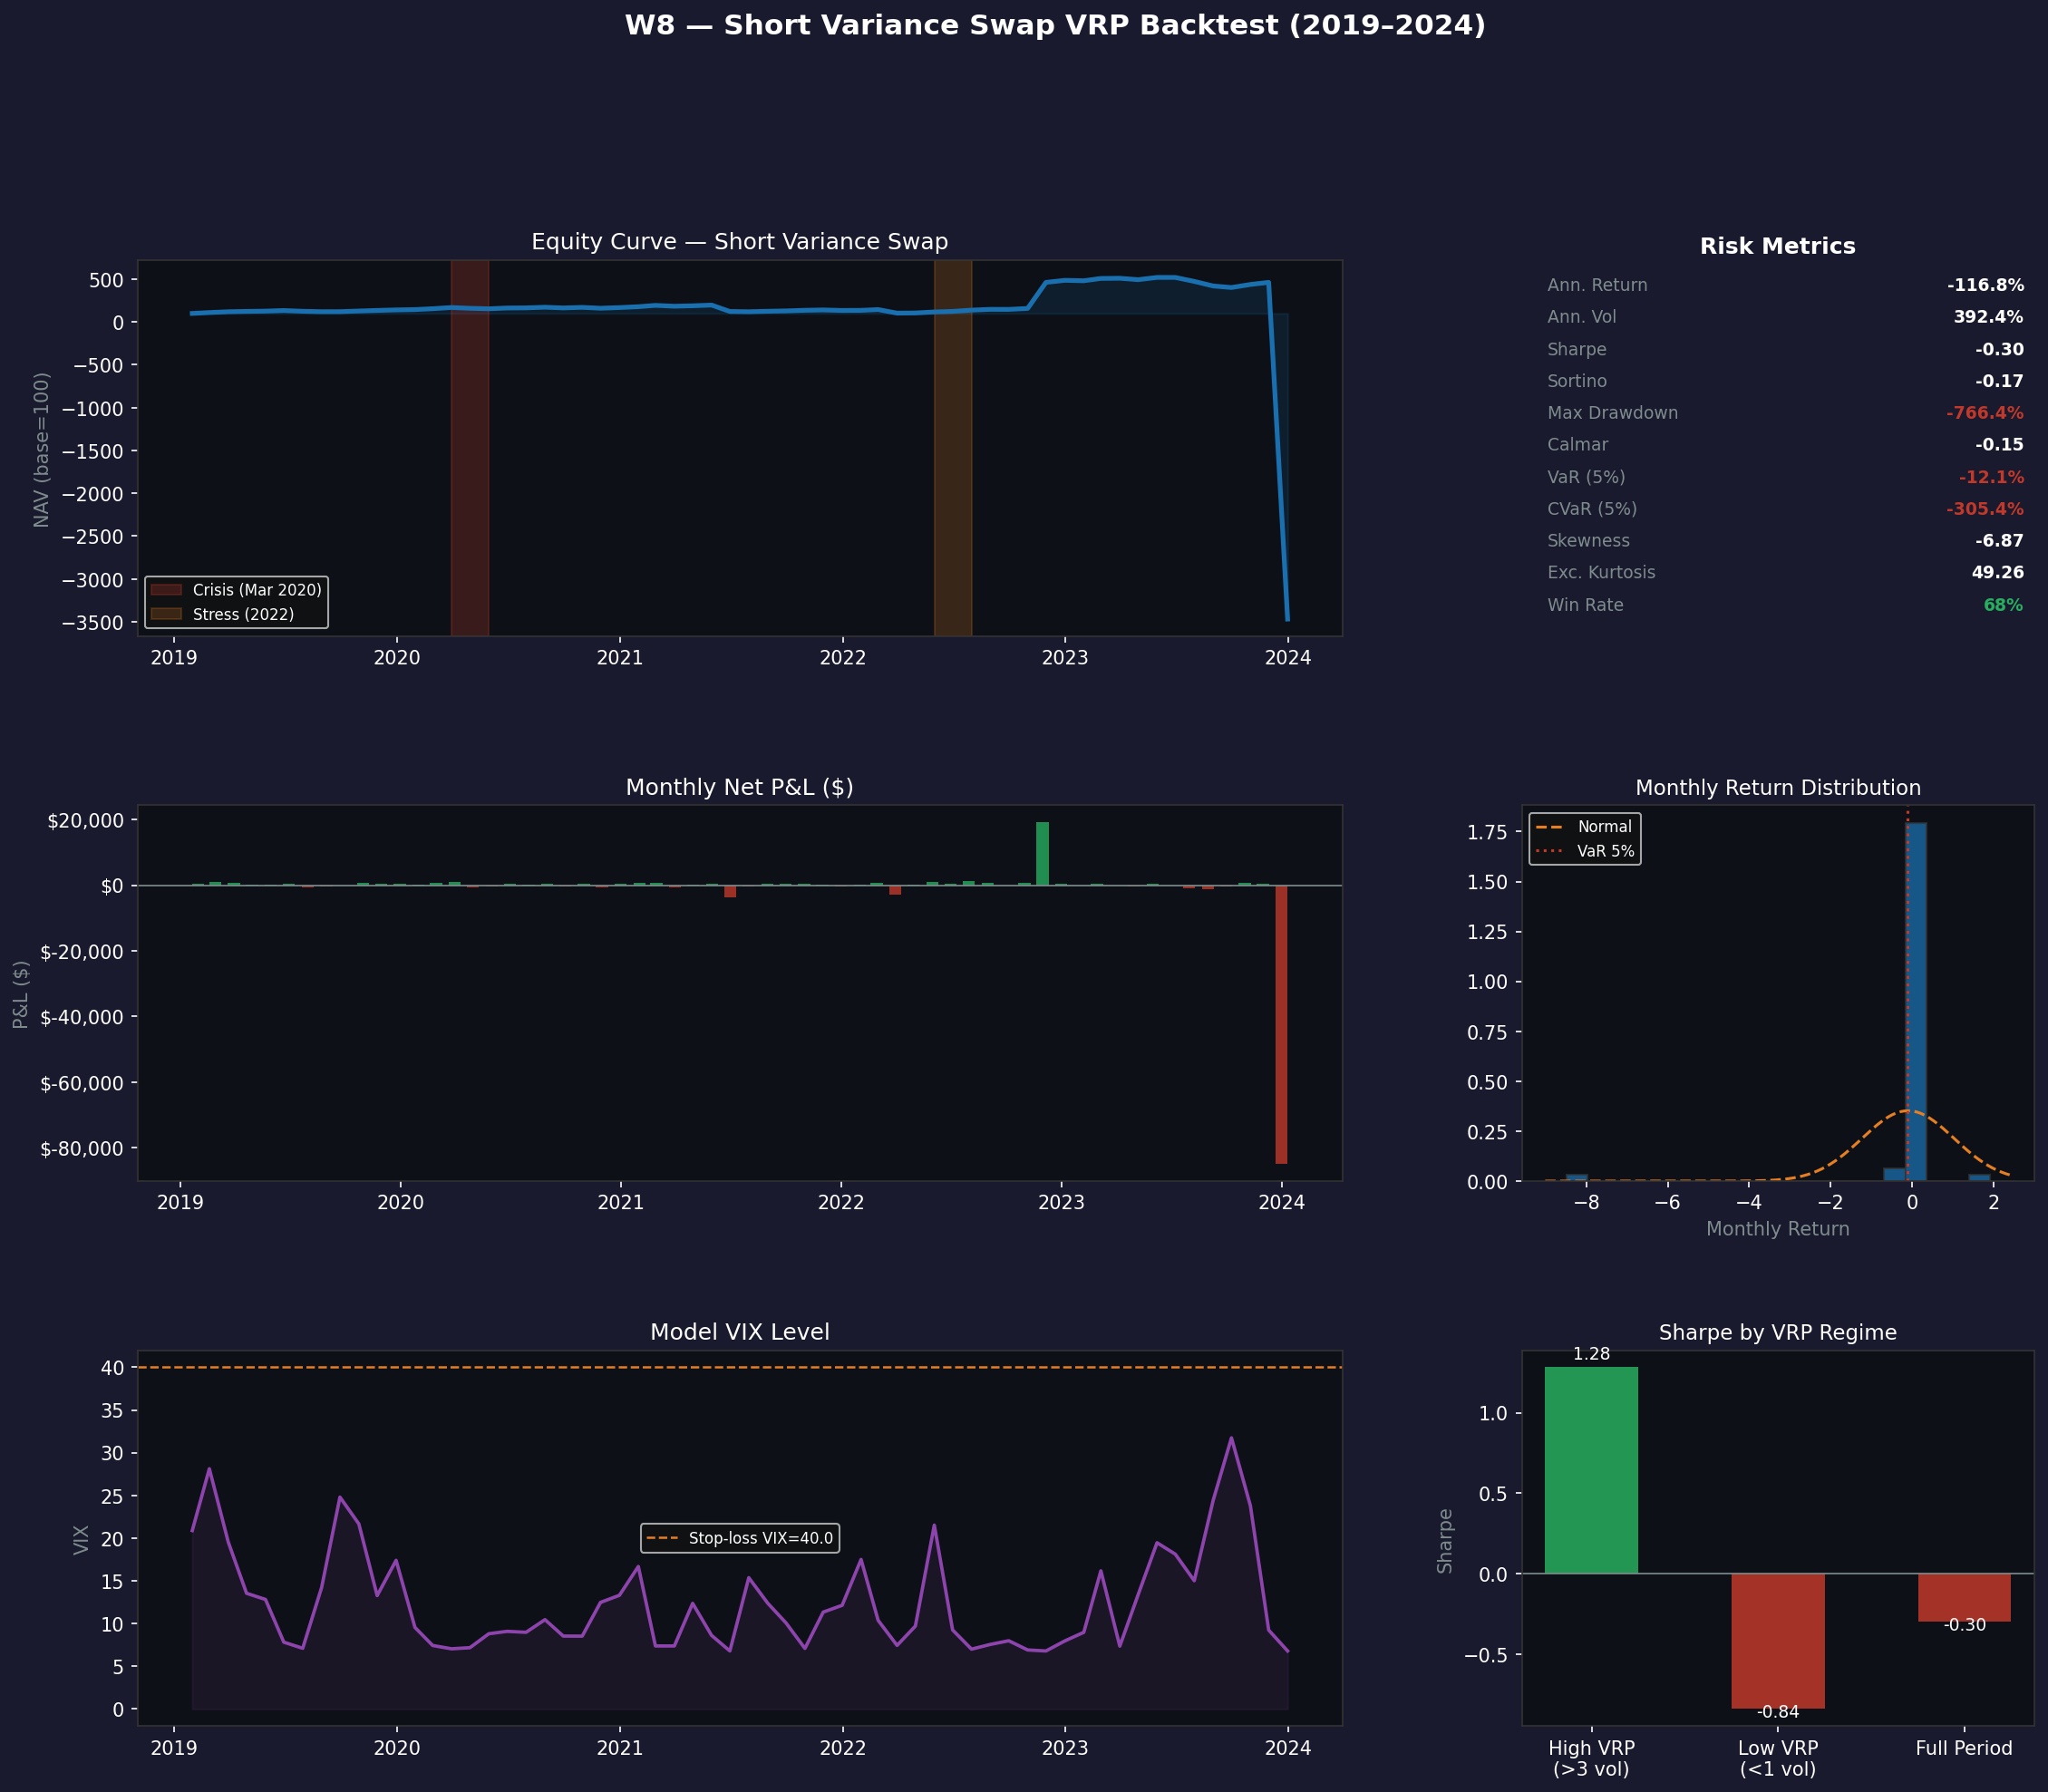
\includegraphics[width=0.88\textwidth]{figures/w8_backtest.png}
    \caption{Backtest performance of the volatility risk premium strategy. The figure summarises the cumulative behaviour of the strategy across the analysed period.}
    \label{fig:w8_backtest}
\end{figure}

Figure~\ref{fig:w8_daily_pnl} shows the daily P\&L behaviour of the strategy.

\begin{figure}[htbp]
    \centering
    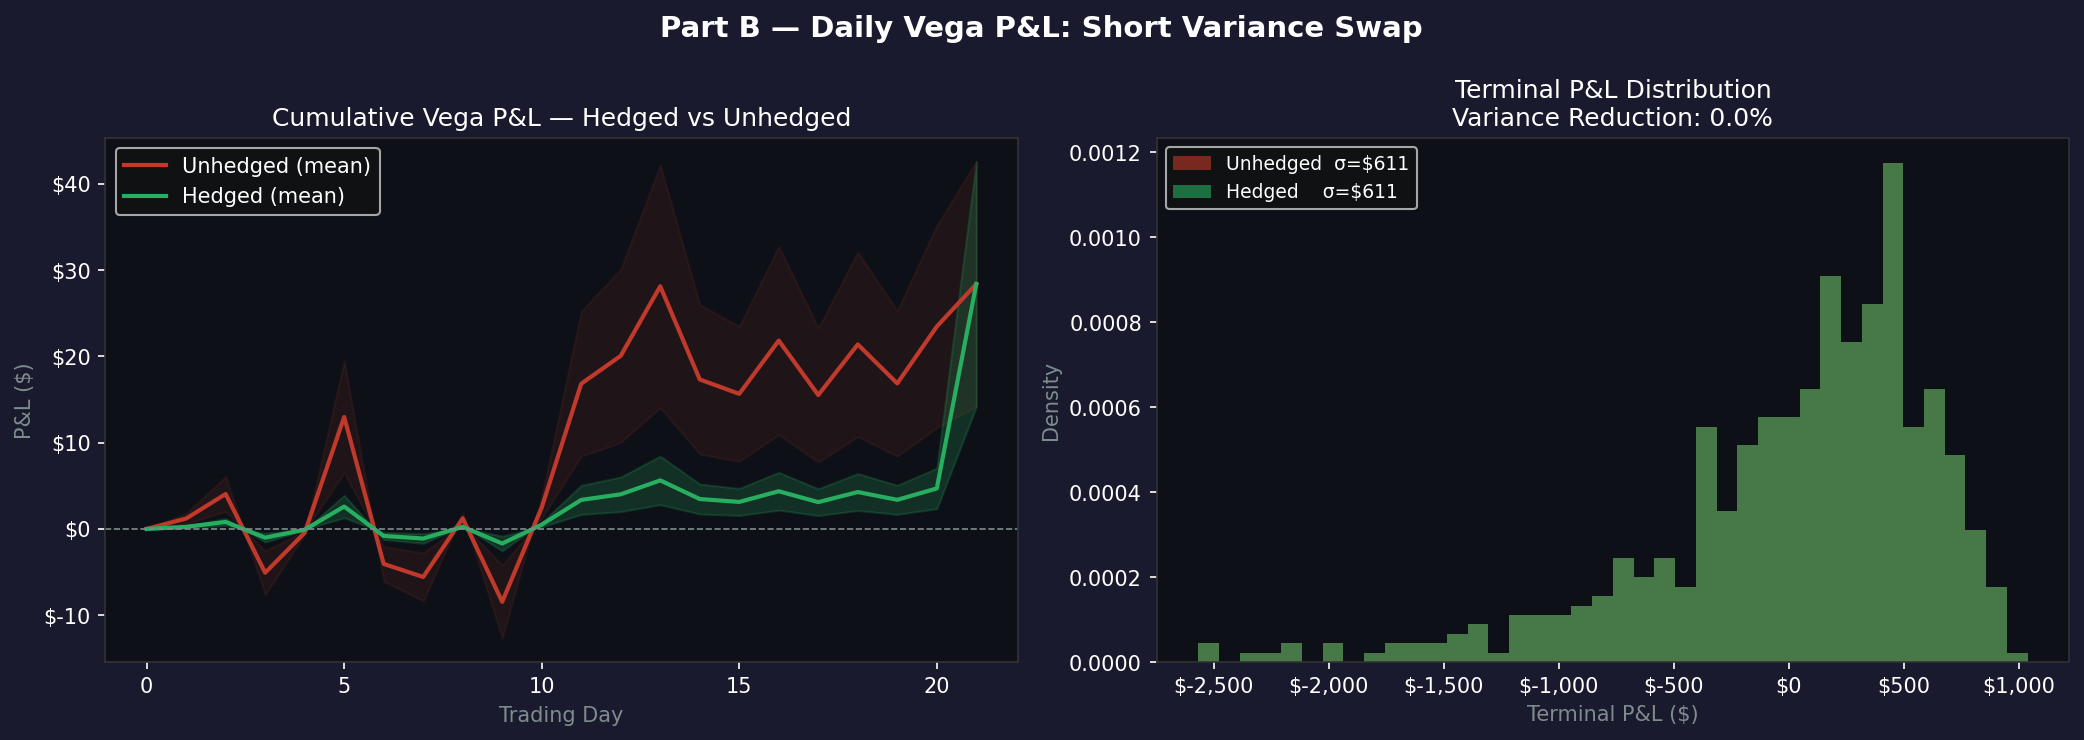
\includegraphics[width=0.88\textwidth]{figures/w8_daily_pnl.png}
    \caption{Daily P\&L of the volatility risk premium strategy. The figure illustrates the time-series behaviour and stress sensitivity of the strategy.}
    \label{fig:w8_daily_pnl}
\end{figure}

The W8 metrics are summarised in Table~\ref{tab:w8_vrp_metrics}.

\begin{table}[htbp]
\centering
\begin{tabular}{lccc}
\toprule
Metric & Full Period & High VRP Regime & Low VRP Regime \\
\midrule
Annual return & -- & 2.154 & -- \\
Annual volatility & 3.925 & 1.218 & 6.102 \\
Sharpe ratio & -- & 1.768 & -- \\
Maximum drawdown & -7.664 & 0.000 & -2.763 \\
VaR 5\% & -0.121 & 0.039 & -0.369 \\
CVaR 5\% & -3.054 & 0.035 & -4.438 \\
Skewness & -7.044 & 5.264 & -4.775 \\
Kurtosis & 53.708 & 27.794 & 22.855 \\
Observations & 60 & 28 & 23 \\
\bottomrule
\end{tabular}
\caption{W8 volatility risk premium backtest metrics across regimes. Empty entries correspond to metrics not reported in the generated output file.}
\label{tab:w8_vrp_metrics}
\end{table}

The high-VRP regime shows the strongest risk-adjusted profile, with a reported Sharpe ratio of approximately \(1.77\), annual return of approximately \(2.15\), and annual volatility of approximately \(1.22\). However, the full-period metrics also show strong negative skewness and high kurtosis, indicating that volatility-selling strategies carry significant tail risk.

Figure~\ref{fig:w8_metrics_dashboard} summarises the W8 strategy metrics visually.

\begin{figure}[htbp]
    \centering
    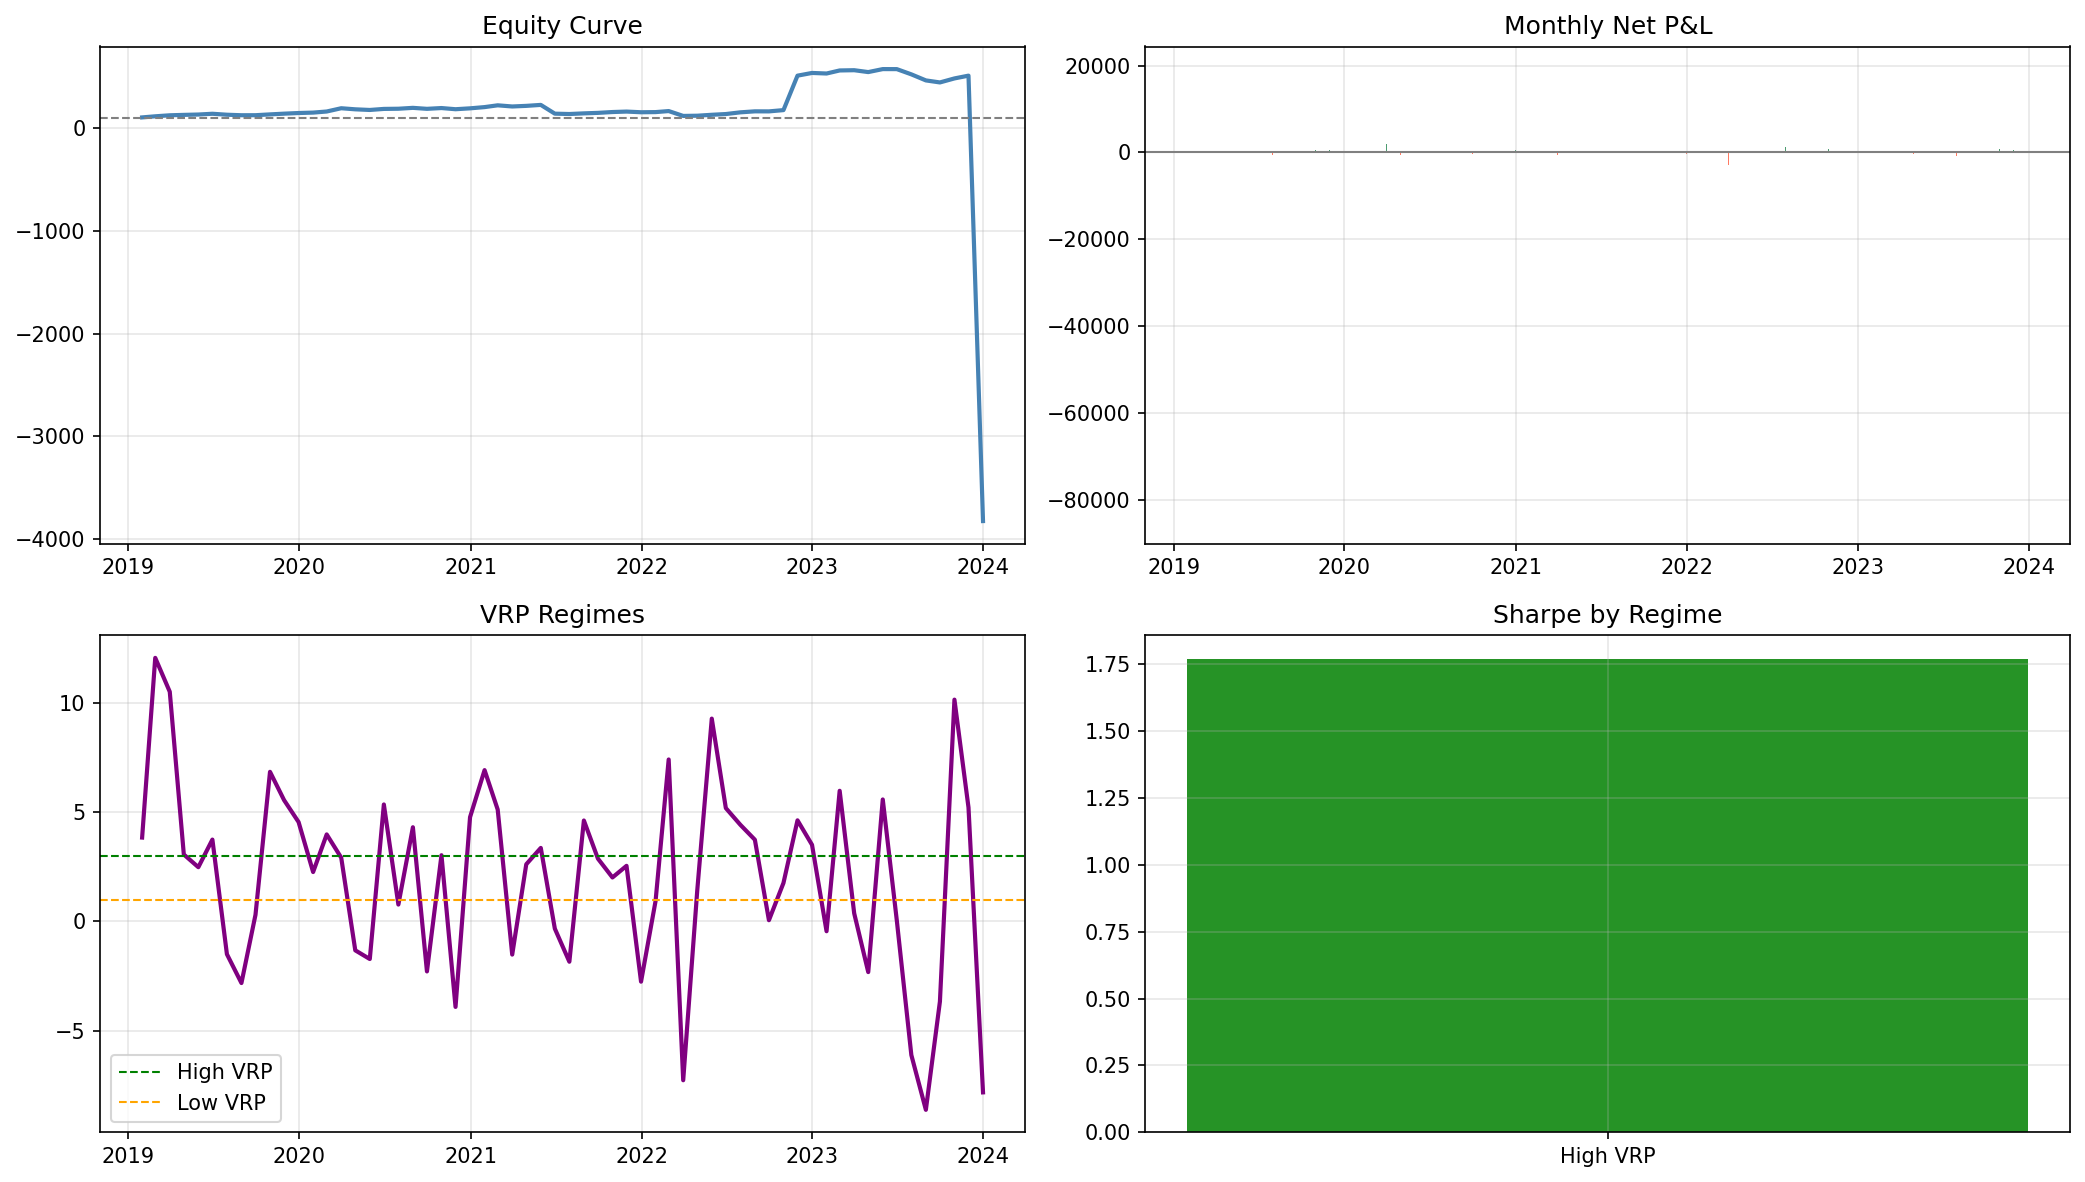
\includegraphics[width=0.88\textwidth]{figures/w8_metrics_dashboard.png}
    \caption{W8 risk and performance dashboard for the volatility risk premium strategy. The dashboard summarises return, volatility, drawdown, and tail-risk behaviour across regimes.}
    \label{fig:w8_metrics_dashboard}
\end{figure}

The W8 results are consistent with the economic interpretation developed earlier in the paper. Volatility risk premium strategies can perform well when implied variance is high relative to expected realised variance, but they remain exposed to severe losses during volatility spikes and crisis periods. Therefore, performance evaluation must include not only average returns and Sharpe ratios, but also drawdowns, tail losses, skewness, and regime dependence.

\subsection{Model-Free Hedging Output}

The W8 outputs also include a model-free hedge diagnostic. Figure~\ref{fig:w8_model_free_hedge} summarises the generated hedge output.

\begin{figure}[htbp]
    \centering
    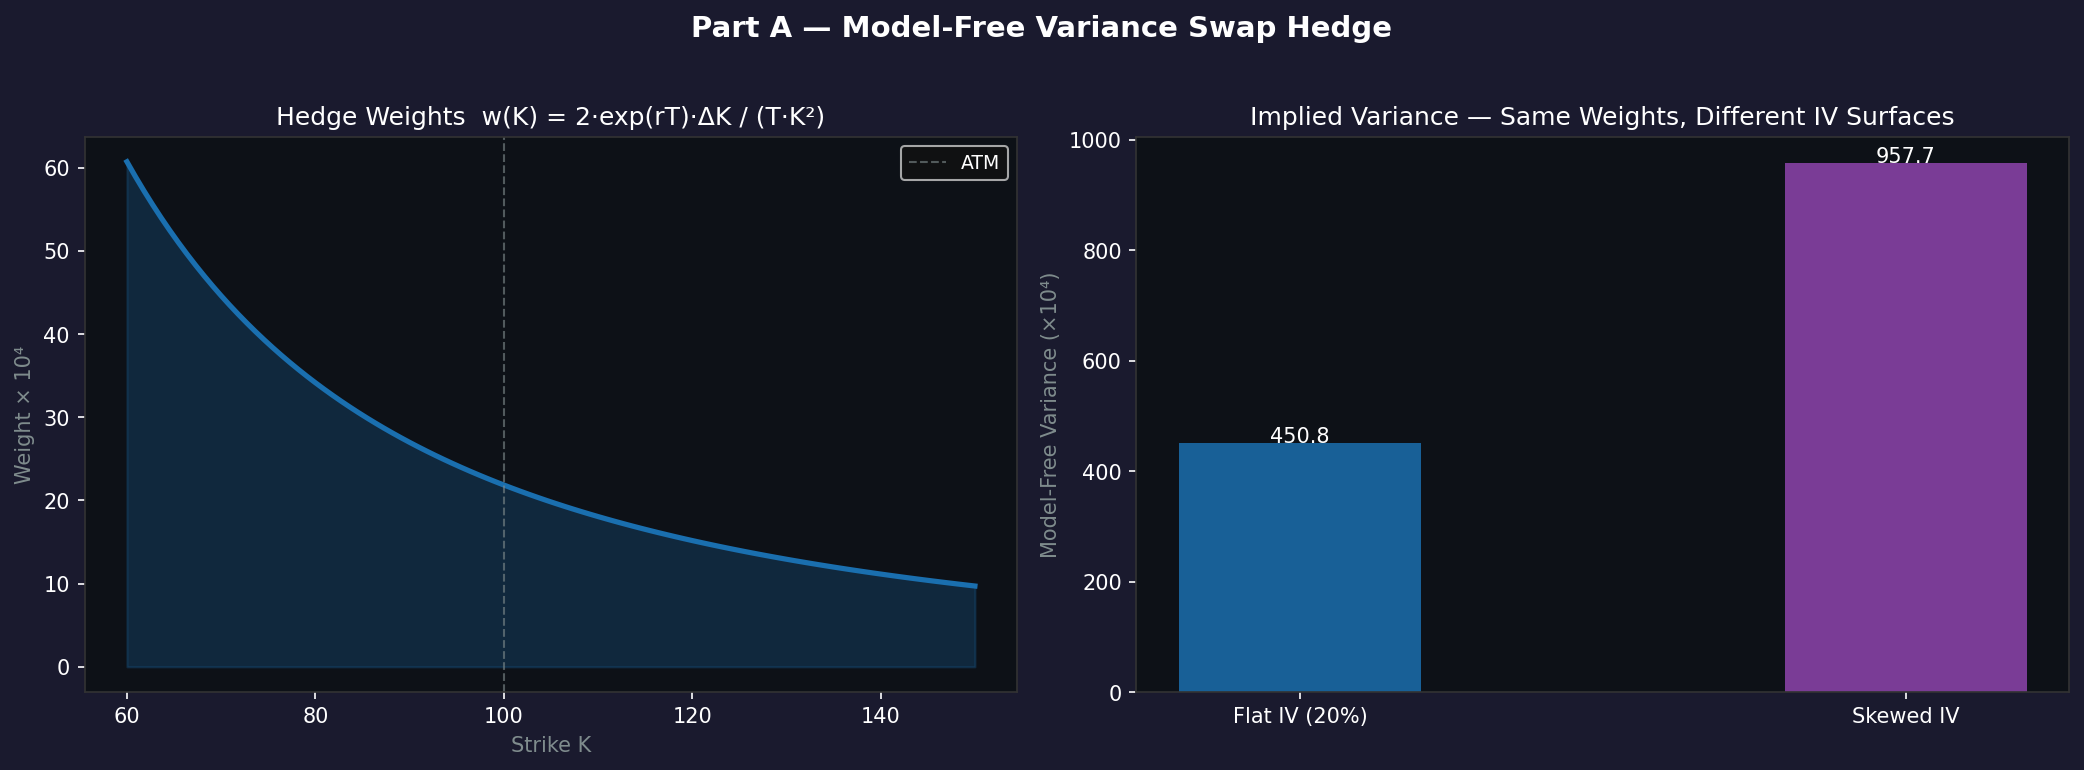
\includegraphics[width=0.88\textwidth]{figures/w8_model_free_hedge.png}
    \caption{Model-free hedging diagnostic generated in W8. The figure provides an additional view of strategy risk management and hedge behaviour.}
    \label{fig:w8_model_free_hedge}
\end{figure}

The inclusion of hedge diagnostics is important because volatility strategies cannot be evaluated only by their average return. A strategy may appear profitable in normal regimes but fail during volatility spikes if hedging is weak or if tail exposure is not controlled.

\subsection{Integrated Interpretation across W3--W8}

The completed project forms a coherent pipeline. W3 provides a Monte Carlo simulation engine for stochastic variance and VIX-type payoffs. W4 provides a faster COS pricing engine based on the CIR characteristic function. W5 introduces real market data and volatility risk premium estimation. W6 demonstrates the calibration trade-off between SPX and VIX markets. W7 explains the structural difference between SPX and VIX volatility smiles. W8 evaluates the practical risk-return behaviour of a volatility risk premium strategy.

The central conclusion is that volatility can be treated as a tradable asset class, but it requires careful modelling. Simple one-factor stochastic volatility models are useful for theory and implementation, but they face limitations in joint calibration and empirical strategy design. Numerical pricing, calibration, smile analysis, and backtesting must therefore be interpreted together rather than as separate tasks.